%------------------------COMEÇA PROPOSTA-----------------
\chapter{Proposta}
\label{cap:proposta}
O seguinte capítulo tem como objetivo elucidar a proposta deste trabalho, que é a criação de um jogo multijogador de tiro em 
primeira pessoa 3D estilo arena. Ao longo do capítulo serão apresentados os seguintes tópicos :
\begin{itemize}
    \item Documento de Game Design (GDD) \footnote{GDD: \textit{Game Design Document}, um documento de projeto do conceito do jogo, descrevendo suas características e elementos.} simplificado, descrevendo uma visão geral do jogo, aspectos de sua jogabilidade e de suas arenas (\textit{Level Design})\footnote{\textit{Level Design} : Projeto de níveis, refere-se a elaboração de cenários e fases de um jogo, inclui o projeto de inimigos, rotas e obstáculos.} e características de seu estilo de arte;
    \item Descrição das ferramentas utilizadas;
    \item Planejamento do desenvolvimento para o Trabalho de Conclusão de Curso 2.
\end{itemize}

\section{GDD }\label{sec:propostaGDD}

Nesta seção será feito um Documento de Game Design simplificado abordando os principais aspectos do jogo proposto.

\subsection{Visão geral}\label{subsec:GDDVisaoGeral}
O jogo proposto Jump'n'Shoot se trata de um multijogador de tiro em primeira pessoa com elementos de arena. Neste jogo, cada jogador controla um personagem , movimentando-se pelo mapa e coletando armas. Cada jogador faz parte de um time, azul ou vermelho, e pode ser identificado pela cor do seu personagem. O ciclo de interação com o jogo, também conhecido como \textit{core gameplay loop} será de andar, procurar armas, disparar contra adversários e desviar de seus projéteis. O jogo não contará com um sistema de progressão como níveis, conteúdo desbloqueável e conquistas.

O objetivo do jogo é eliminar os outros jogadores e ganhar pontos cumprindo objetivos segundo cada modo de jogo. Algumas variáveis como tempo máximo da partida, número de vidas e pontos para ganhar serão definidos antes da partida começar, pelo usuário hospedeiro \footnote{Jogador hospedeiro : Jogador que cumpre a função de servidor , ou hospedeiro, como descrito na Figura \ref{fig:p2p} }.

\subsection{Jogabilidade }\label{subsec:GDDJogabilidade}
A jogabilidade de um jogo pode ser definida segundo vários aspectos, sendo os principais : elementos, objetivos, controles e progressão. A seguir, serão definidos alguns desses aspectos para o jogo proposto.

\subsection{Elementos do \textit{Core Gameplay Loop}}\label{subsec:coreGameplay}
Os elementos constituintes do \textit{core gameplay loop} no jogo proposto são :
\begin{itemize}
    \item Movimentação: O jogador movimenta-se para frente, para trás e para os lados, podendo andar ou correr.
    \item Mira: O jogador manipula o mouse ou o analógico direito do controlador de jogo para regular a orientação da mira da arma ou seja, a posição em que os disparos serão feitos.
    \item Pulo: O jogador realiza um salto, deslocando-se para cima.
    \item Pulo duplo: O jogador pode pular uma segunda vez.
    \item Disparo: O jogador pode realizar disparos com suas armas e atingir outros jogadores. Todos os jogadores contam com uma arma padrão de munição ilimitada desde o surgimento; as outras armas devem ser coletadas no cenário e têm munição limitada. 
    \item Plataforma : As plataformas são blocos suspensos no ar que ficam posicionadas no mapa com o propósito de viabilizar o acesso aos itens coletáveis do pelo jogador. Uma plataforma pode ser fixa, móvel e/ou quebradiça.
    \item Plataforma móvel: Uma plataforma pode mover-se segundo um determinado padrão, para cima e para baixo como um elevador ou para os lados.
    \item Plataforma quebradiça: Uma plataforma quebradiça se quebrará após um curto período de tempo no momento em que um jogador entrar em contato.
    \item Plataforma de impulso: O jogador posiciona-se sobre plataformas especias no chão do mapa que impulsionam seu personagem para frente e para cima, sendo lançado ao ar.
    \item Pontos de vitalidade: Cada jogador conta com pontos de vitalidade, que são decrementados ao ser acertado por projéteis de outros jogadores. Quando tal valor chega à zero, o contador de vidas do jogador é diminuído em uma unidade.
    \item Ponto de nascimento: Os jogadores surgem e ressurgem no mapa de jogo em posições pré determinadas.
    \item Vidas limitadas: O jogador conta com um número de vidas, que são diminuídas sempre que seus pontos de vitalidade chegarem à zero. Caso o jogador ainda tenha vidas disponíveis, ele poderá renascer após um período em segundos determinado previamente pelo hospedeiro da partida.
    \item Coleta de itens: O jogador pode coletar itens no cenário movimentando-se através deles. Os itens disponíveis para coleta são: pontos de vitalidade, vidas, armas, melhoria temporária de velocidade, melhoria temporária de dano e a bandeira no modo "capture a bandeira".
    \item Melhoria temporária de dano: Quando coletado por um jogador, durante os próximos 15 segundos o jogador causa dano dobrado nos pontos de vitalidade dos outros jogadores.
    \item Melhoria temporária de velocidade: Quando coletado por um jogador, durante os próximos 15 segundos o jogador se movimenta mais rápido. 
\end{itemize}

\subsection{Modos de jogo}\label{subsec:modosDeJogo}
Além dos elementos básicos, o jogo terá diferentes modos de jogo, com regras e condições de vitória diferentes.São estes:
\begin{itemize}
    \item Capture a bandeira: Os jogadores são divididos em equipes e uma área do mapa é designada a cada time, onde suas respectivas bandeiras aparecem. O objetivo é capturar a bandeira do time inimigo e trazer de volta à sua base. Cada captura vale pontos e ao fim de um período de tempo pré determinado , ou quando um time contabilizar um certo valor em pontos, a equipe com mais pontos é declarada vencedora. Os jogadores também podem renascer livremente, pois não há contagem de vidas. 
    \item Mata-mata em equipe: Neste modo o objetivo é contabilizar pontos eliminando os jogadores da equipe inimiga, até que um dos times não tenha mais jogadores com vidas ou o tempo se esgote. O primeiro time a alcançar a marca ou o que obtiver mais pontos ao fim do tempo vence.
    \item Rei do pedaço: Os jogadores são divididos em times, e há uma área neutra no meio do mapa de jogo. Cada time ganha pontos a cada unidade de tempo enquanto tem pelo menos um aliado tocando essa área neutra. O jogo acaba quando um dos times chegar à contagem máxima de pontos; tal time é então declarado vencedor.
\end{itemize}

\subsection{Armas do jogo}
As armas disponíveis para cada jogador são:
\begin{itemize}
    \item Pistola: Arma padrão com munição infinita, disponível em todos os modos de jogo desde o surgimento do personagem. Esta arma causa menos dano e tem uma taxa de disparo mais lenta.
    \item Rifle automático: Arma de repetição com alta cadência de projéteis; causa mais dano do que a pistola. 
    \item Canhão laser: Uma arma de precisão que dispara um raio concentrado , causando muito dano porém com uma baixa taxa de disparo. 
    \item Lança-foguetes: Dispara um projétil lento que explode ao colidir com o cenário ou outro jogador, causando dano moderado no entorno da área de impacto.
\end{itemize}

\subsection{Controles do jogo}
A forma que o jogador terá disponível para controlar seu personagem é por meio do mouse e teclado ou controlador de jogo. A seguir será exposto uma imagem do mapeamento de teclas bem como uma tabela apresentando um resumo dos controles e suas respectivas ações.

\begin{figure}[htb]%% Ambiente figure
    %\captionsetup{width=0.55\textwidth}%% Largura da legenda
    \caption{Mapeamento de controle do jogo no mouse e teclado e \textit{joystick}.}%% Legenda
    \label{fig:mapeamento}%% Rótulo
    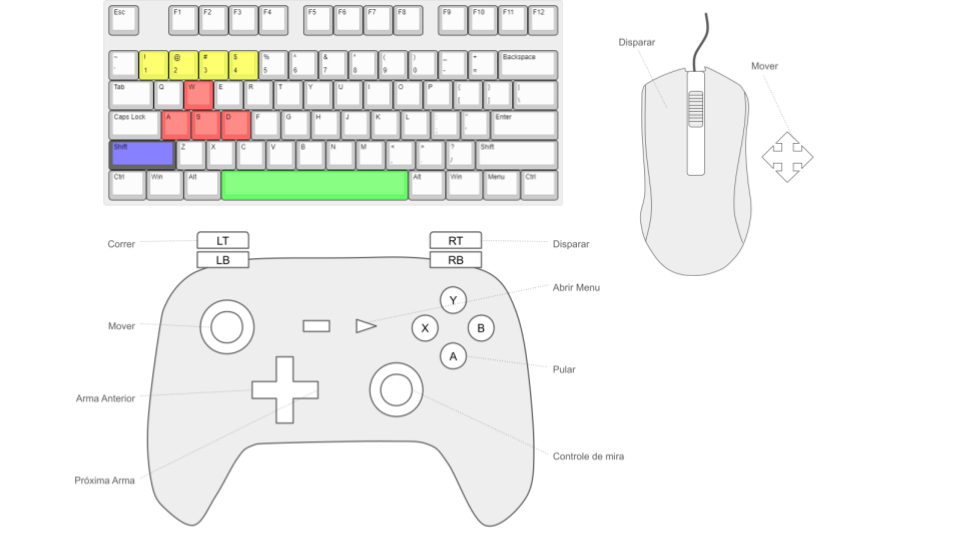
\includegraphics[scale=0.6]{imgs/layout_geral.png}%% Dimensões e localização
    \fonte{Autoria própria (2023)}%% Fonte
    \end{figure}

\begin{table}[]
\centering

\begin{tabular}{|c|c|c|}
  \hline
  \textbf{Teclado} & \textbf{Gamepad} & \textbf{Ação} \\
  \hline
  W &Analógico Esquerdo & Movimenta-se para frente \\
  \hline
  S & Analógico Esquerdo & Movimenta-se para trás \\
  \hline
  A & Analógico Esquerdo &Movimenta-se para a esquerda \\
  \hline
  D & Analógico Esquerdo &Movimenta-se para a direita \\
  \hline
  SHIFT & Gatilho Esquerdo &Entra no modo corrida  \\
  \hline
  Espaço & Botão A &Realiza um salto \\
  \hline
  1,2,3,4 & Seta Direita e Esquerda &Troca entre as armas \\
  \hline
  ESC &Botão Start & Abre o menu do jogo \\
  \hline
  Botão esq. do mouse &Botão Direito & Realiza um disparo \\
  \hline
  Movimentar o mouse & Analógico Direito &Gira a câmera na direção do movimento.\\
  \hline
\end{tabular}
\caption{Resumo dos controles do jogo.}
\label{tab:mapeamento}
\end{table}
%\caption{Descrição dos controles do jogo.}

\subsection{Interface e fluxo de telas}\label{subsec:interface}
Foi criado um protótipo no software Balsamic Wireframes que descreve o fluxo de interação do jogador com a interface de usuário do jogo. Na Figura \ref{fig:interface} são apresentadas as diferentes telas do jogo, bem como o fluxo de troca entre elas.

 \begin{figure}[htb]
    \caption{Fluxo de interação com a interface do jogo}
    \label{fig:interface}%% Rótulo
    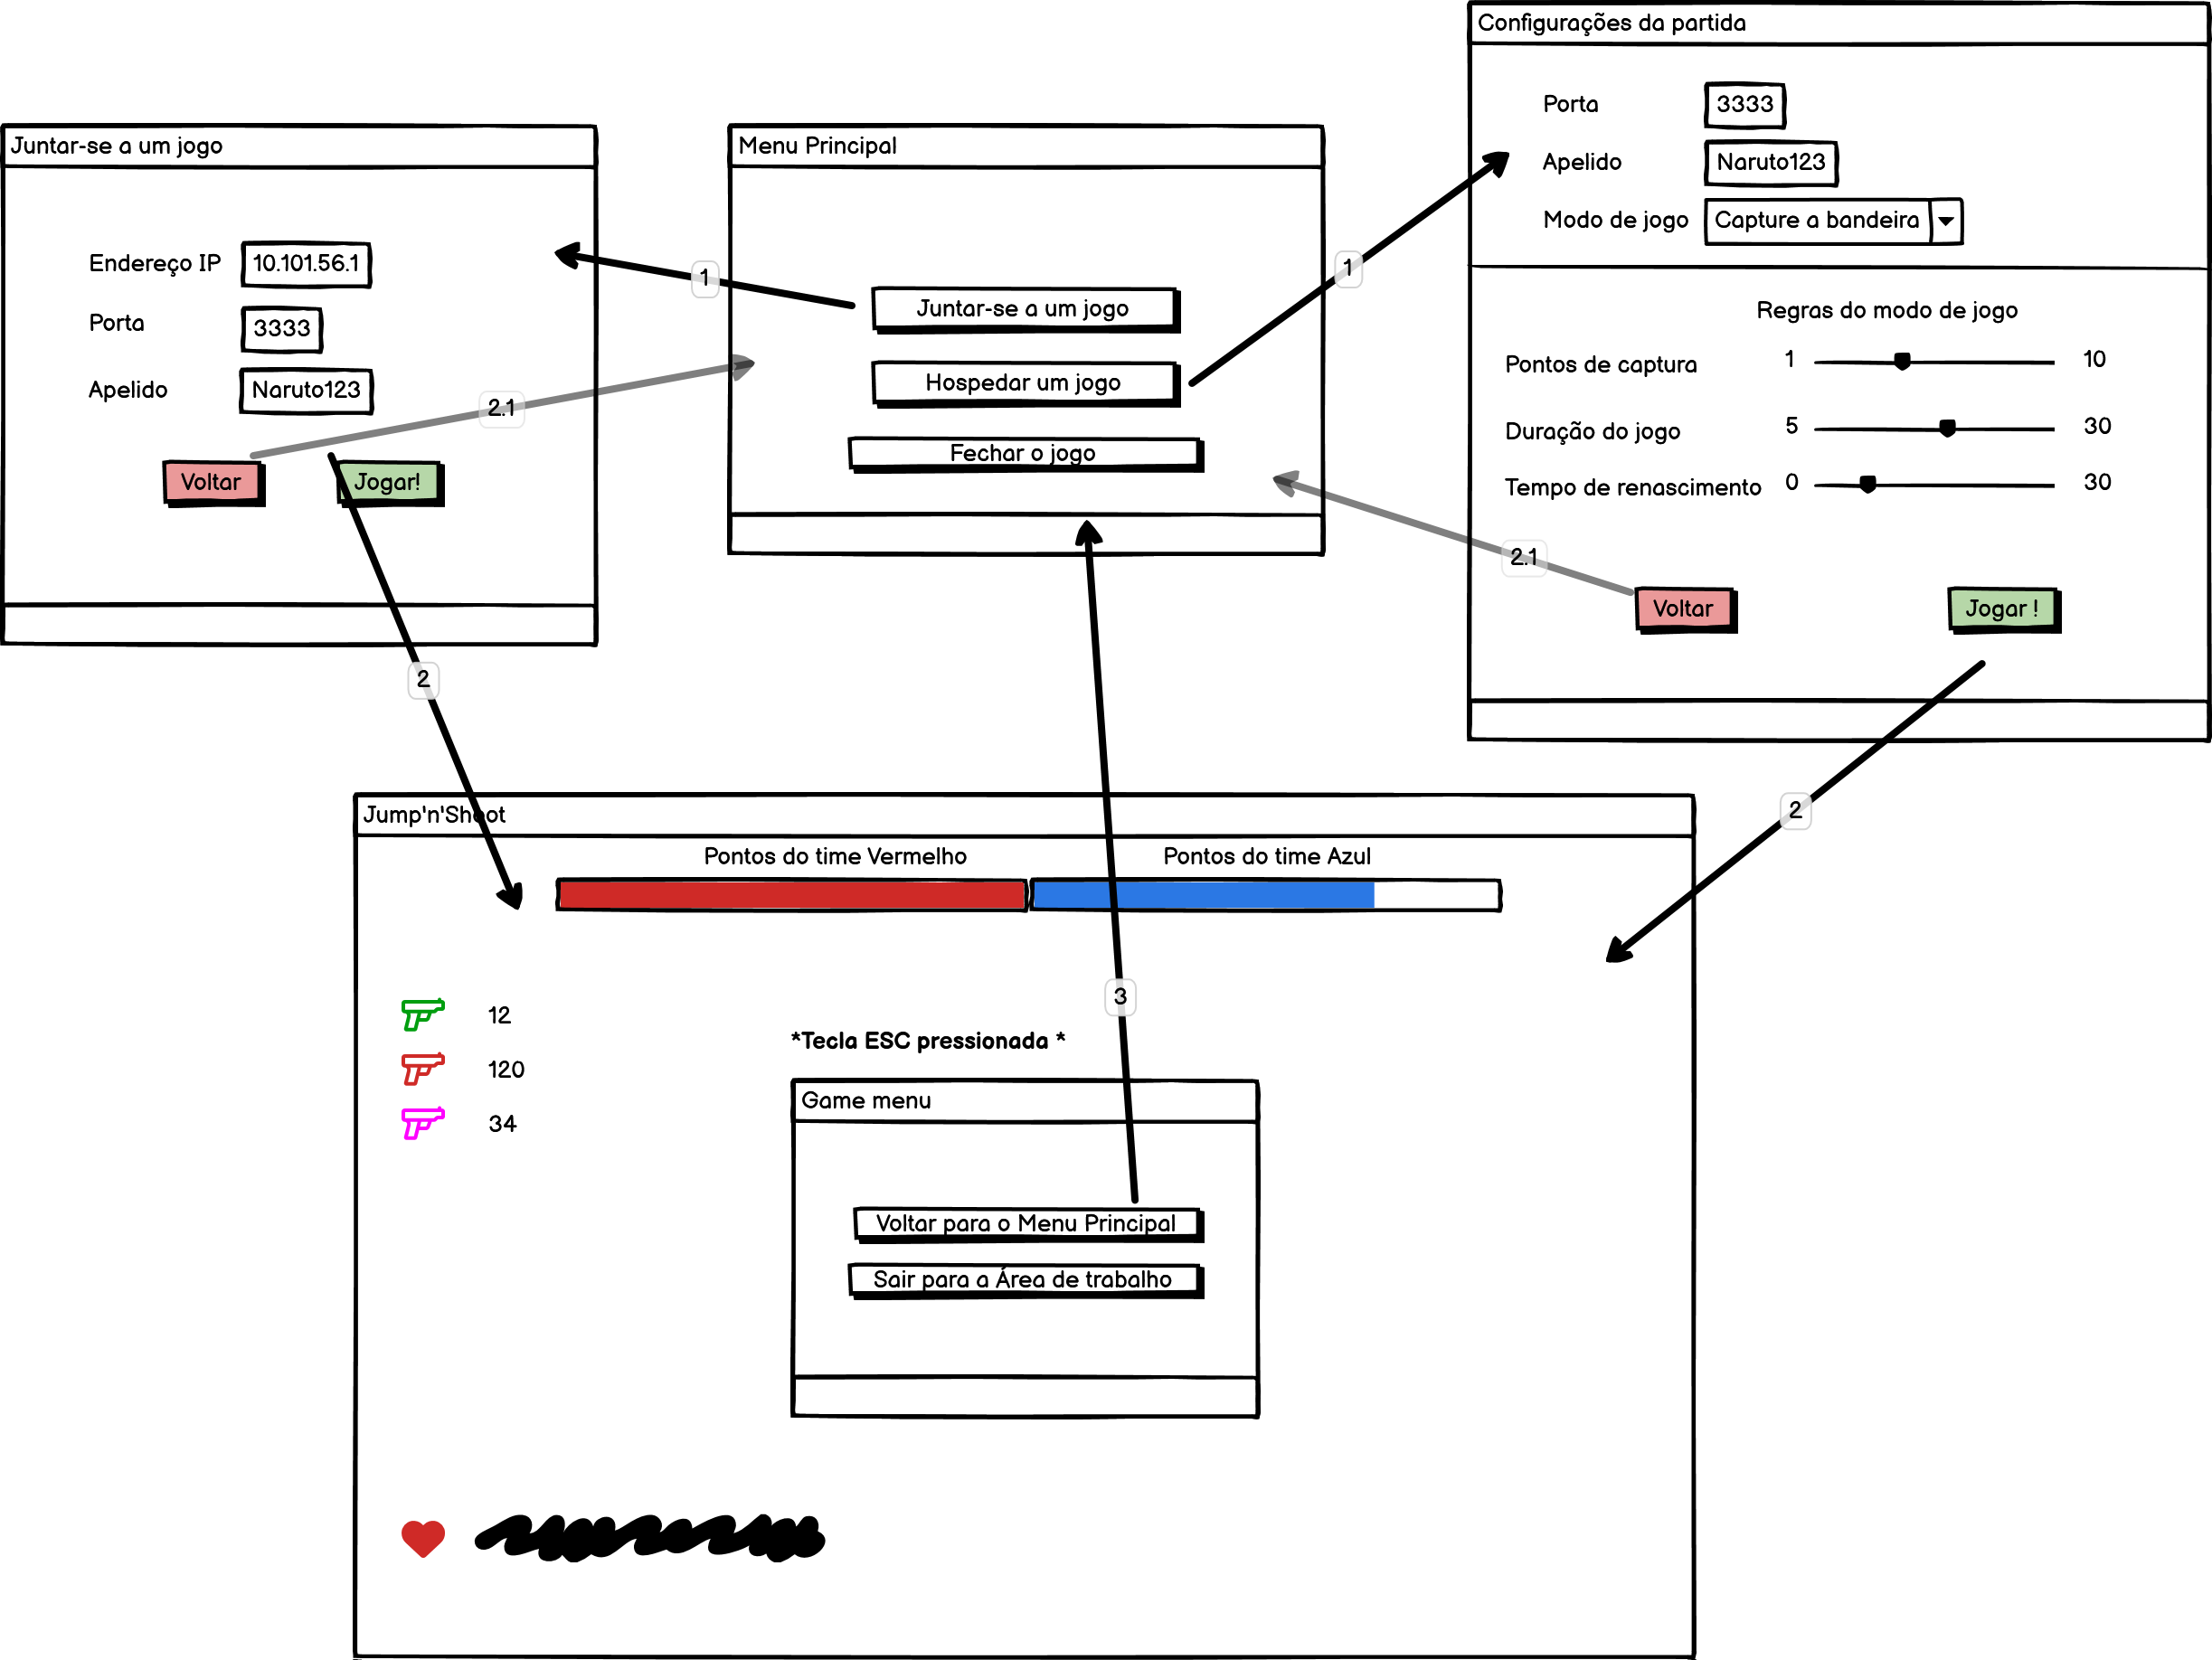
\includegraphics[scale = 0.5]{imgs/interface.png}%% Dimensões e localização
    \fonte{Autoria Própria}
    \end{figure}

Ao abrir o jogo, é apresentado ao usuário a tela do menu principal, que o permite juntar-se a uma partida ou criar a própria. Caso o jogador crie a própria partida, ele escolhe o modo de jogo, as opções e inicia, os demais jogadores devem juntar-se a essa partida criada, fazendo a escolha dos parâmetros de conexão na tela de "Juntar-se a partida". Uma vez que o jogo comece, o usuário pode apertar a tecla de escape a qualquer momento e escolher entre voltar ao menu e fechar o jogo.
    

\subsection{Level Design}\label{subsec:levelDesign}
O \textit{Level Design} desempenha um papel crucial na experiência de um jogo. É necessário entender as características que compõe o jogo que se pretende criar, pois o que seria uma boa decisão de \textit{level design} em um gênero de jogo pode tornar frustrante para o jogador em outro gênero. Isso é especialmente verdade quando consideramos as diferenças entre jogos cooperativos e competitivos. Por exemplo, uma posição que confere grande vantagem e poucos riscos ao jogador contra inimigos controlados por computador em um jogo de jogador único pode ser considerada injusta em um jogo multijogador competitivo, tornado a experiência desagradável.

A fim de realizar testes de ideias de \textit{level design} e empregando alguns padrões de design propostos por \cite{Hullett2010}, foi elaborado o protótipo de um mapa do jogo considerando o modo "Capture a Bandeira". Esse mapa foi inspirado em um dos níveis mais conhecidos do jogo Unreal Tournament, o \textit{Facing Worlds}. No protótipo mostrado na Figura \ref{fig:prototipoMapa}, os cilindros coloridos representam os jogadores de cada time, sendo esses time azul e vermelho. Os jogadores de cada time são instanciados na parte central de cada torre e a bandeira fica no entorno da construção. A seguir, será apresentada uma breve descrição de alguns padrões de design, com exemplos indicados por marcadores na Figura \ref{fig:prototipoMapa} que exibe o protótipo.
\begin{itemize}
    \item Mapa simétrico: Uma das formas mais simples e justas de se criar um cenário para um jogo FPS competitivo é utilizar mapas simétricos, desta forma cada time terá acesso aos mesmos recursos e possibilidades de jogadas. A principal desvantagem desta escolha é que o jogador pode confundir o lado do mapa em que está. Uma possível solução para esse problema é utilizar cores distintas em cada lado do mapa , para que estes sejam rapidamente identificáveis pelo jogador. No prótotipo desenvolvido o mapa é simétrico com exceção da área central.
    \item Verticalidade : Um nível de jogo que apresenta verticalidade é aquele que explora as diferentes elevações e camadas dentro do ambiente de jogo. No protótipo, há elementos de verticalidade na plataforma que se move no centro do mapa (A), forçando os jogadores que estão no chão a se preocupar também com inimigos na parte de cima do mapa.
    \item Gargalos : Gargalos ou \textit{choke points} são partes do mapa que direcionam os jogadores à um único ponto de encontro, estimulando o combate e disputa por aquele espaço. No protótipo há a presença de um gargalo no corredor da entrada das bases de cada equipe (B).
    \item Posição de franco-atirador: Também conhecido como \textit{sniper location}, são áreas elevadas no mapa em que os jogadores com armas de longo alcance tem alguma vantagem. A ponte e o topo de cada construção (C) no protótipo são exemplos de \textit{sniper locations}.
    \item Cobertura : Uma cobertura é uma estrutura ou objeto do cenário que oferece proteção contra os projéteis inimigos. Temos como exemplo os pilares a pedra e a pilha de toras de madeira, indicados com o marcador (D).
    \item Rotas Alternativas : Rotas alternativas servem principalmente para diminuir a linearidade dos cenários do jogo, sendo linearidade a característica de um mapa ou fase do jogo em que o jogador só pode navegar de uma maneira. Com mais rotas alternativas, aumenta-se a imprevisibilidade do combate entre os jogadores, o que aumenta a diversidade da jogabilidade. O protótipo desenvolvido permite que os jogadores cheguem ao lado da equipe inimiga utilizando mais de uma rota, sendo essas pelo meio e pela plataforma movediça (A), além de permitir a navegação pela parte central de diferentes formas (E).  
\end{itemize}

% https://users.soe.ucsc.edu/~ejw/papers/hullett-fps-fdg2010.pdf
% https://www.gamedeveloper.com/design/the-visual-guide-to-multiplayer-level-design
% https://www.youtube.com/watch?v=PxpjRuATxKE&ab_channel=GDC
% https://www.youtube.com/watch?v=NhMDTxnzQuA&ab_channel=GDC
% https://medium.com/ironequal/practical-guide-on-first-person-level-design-e187e45c744c


\begin{figure}[htb] % Mudar a imagem para uma visão mais completa do mapa 
    \caption{Mapas de jogo : (a)Protótipo de mapa do modo "capture a bandeira" e (b) \textit{Facing Worlds} do \textit{Unreal Tournament}.} 
	\label{fig:prototipoMapa}
	\centering
	\subfloat[Protótipo]{
		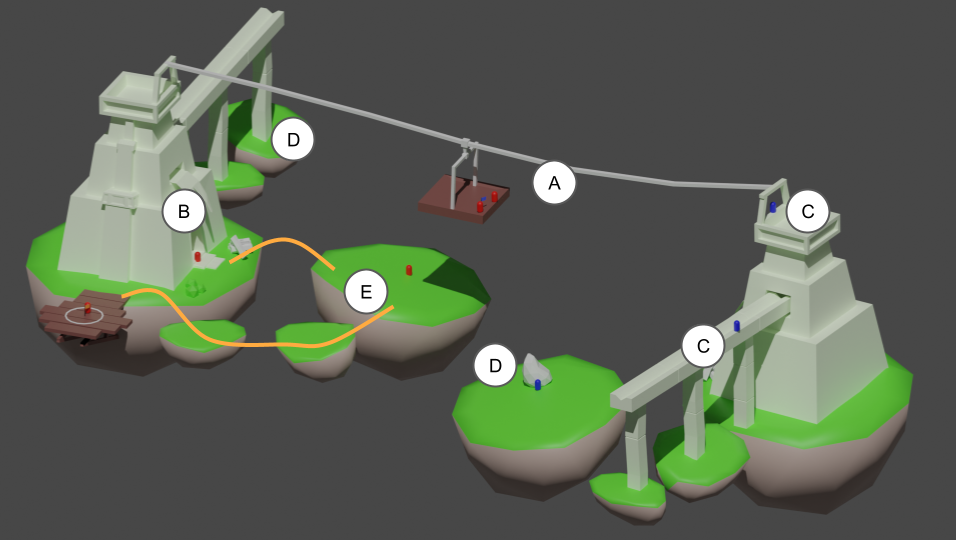
\includegraphics[width=10cm, height=6cm]{imgs/bg_isometric.png} 
        \vspace{0.5cm}


        
	}\hspace{0.15cm} 
	\subfloat[ Mapa "Facing Worlds" do Unreal Tournament ]{
		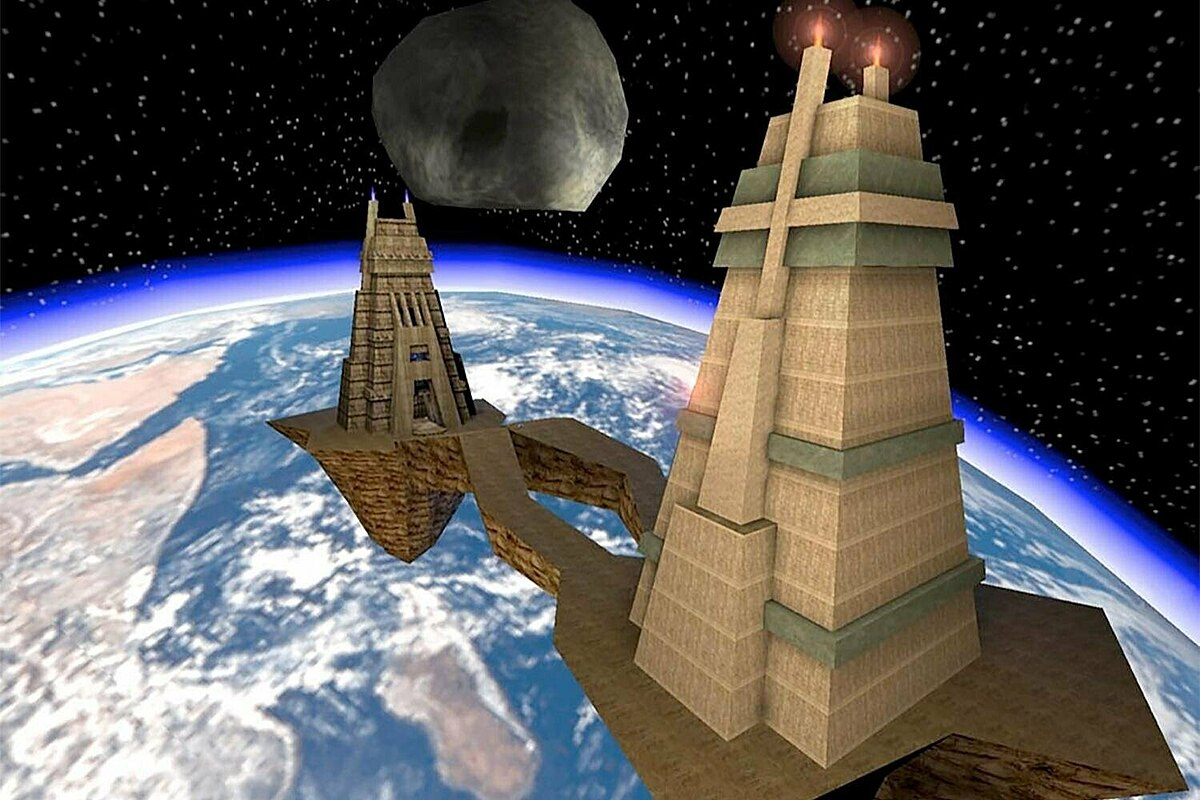
\includegraphics[width=10cm, height=6cm]{imgs/facing_worlds.jpg}
       \vspace{0.5cm}
        

	}
\fonte{a) Autoria Própria , b) Unreal Tournament (1999)}
 \end{figure}


 O principal motivo da escolha desses elementos de design é permitir que os jogadores se enfrentem de formas diferentes. A combinação das diferentes armas e rotas de acesso aos objetivos além das plataformas que se movimentam, faz com que os encontros entre jogadores de times adversários sejam variados e continuem interessantes.

 
 
 \subsection{Arte}\label{subsec:arte}
 O estilo de arte do jogo será cartunesco, com elementos de fantasia e cores vibrantes. Será usado como referência o estilo de arte do jogo \textit{Lovely Planet} \footnote{Lovely planet: Jogo de tiro em primeira pessoa de único jogador, desenvolvido pela quicktequila e lançado em 2014.}, mostrado na Figura \ref{fig:ref:lovelyPlanet}. A motivação para escolha desse estilo é a simplificação dos modelos 3D e texturas que serão utilizadas, além da estética amigável para o público que não gosta de jogos com violência explícita. 

 \begin{figure}[htb]%% Ambiente figure
    %\captionsetup{width=0.55\textwidth}%% Largura da legenda
    \caption{Jogo \textit{Lovely Planet}}
    \label{fig:ref:lovelyPlanet}%% Rótulo
    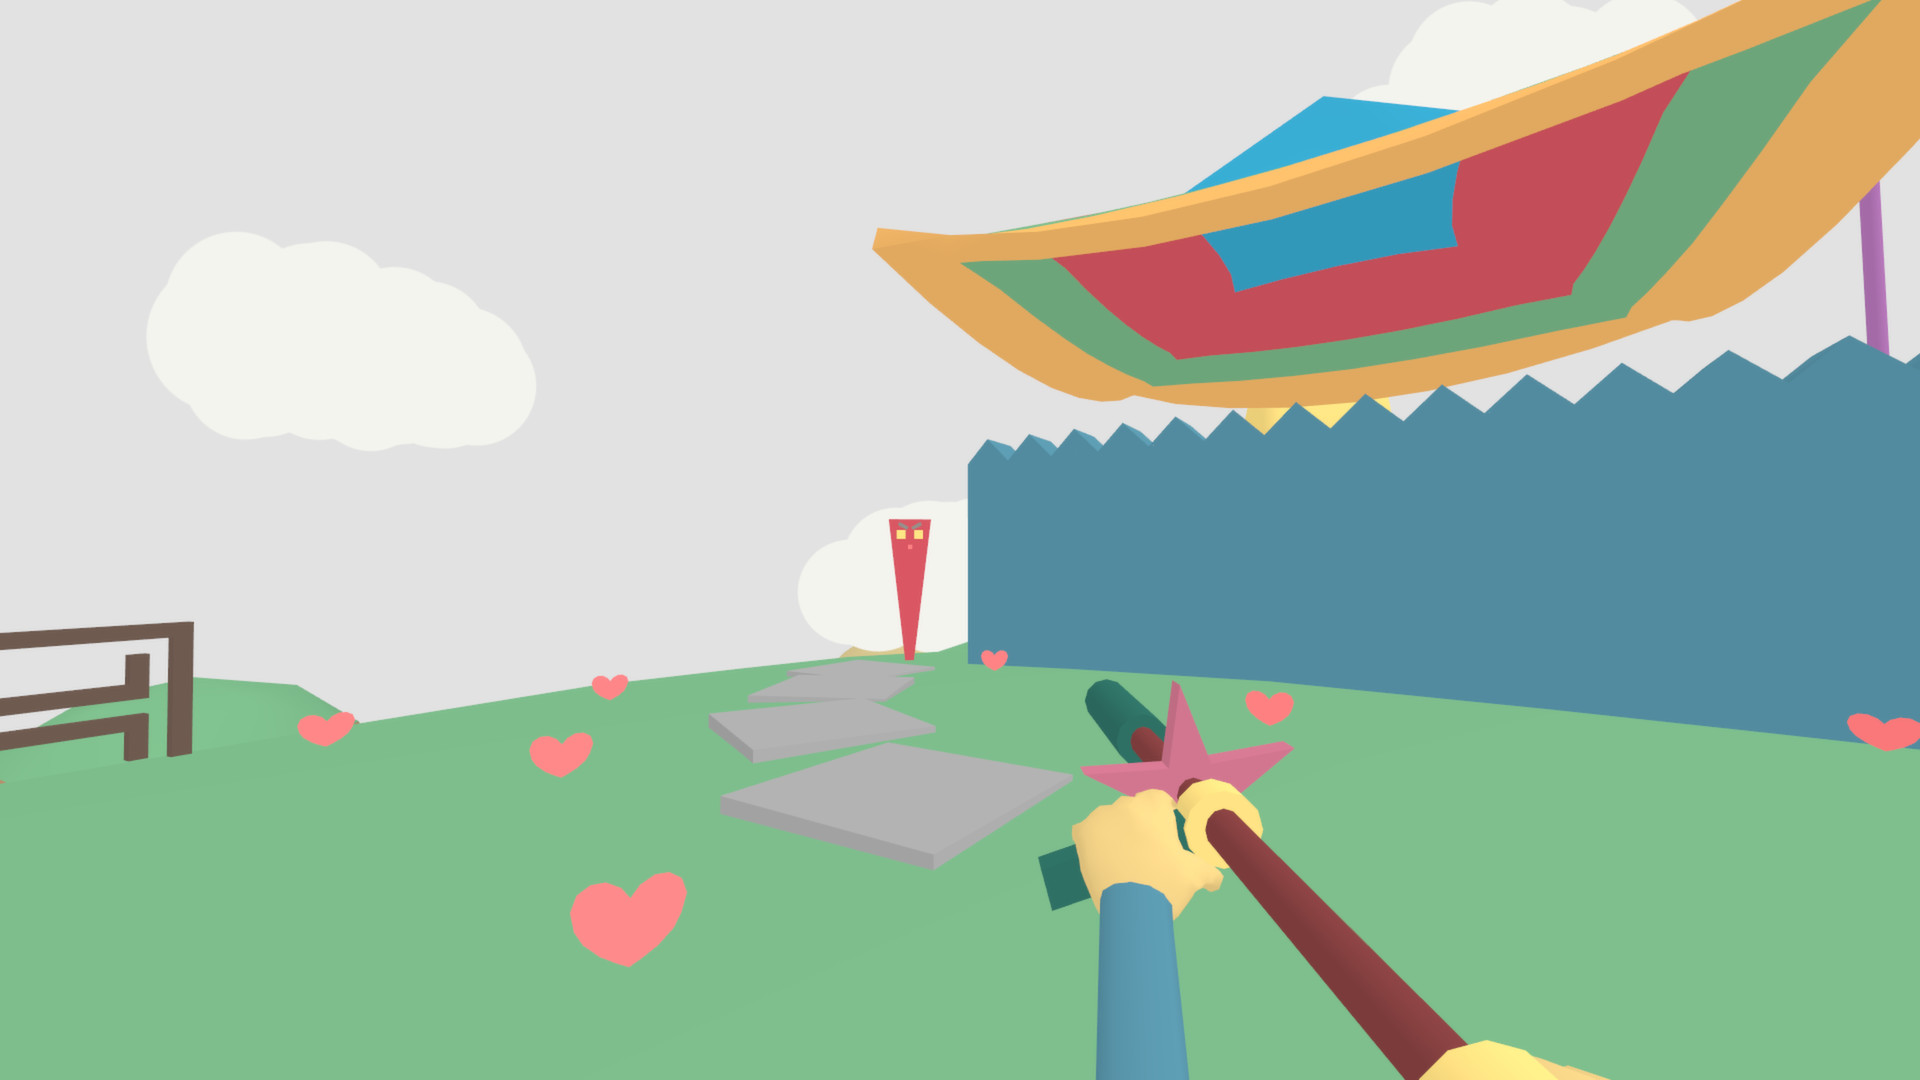
\includegraphics[width=10cm, height=6cm]{imgs/lovelyplanet.jpg}%% Dimensões e localização
    \fonte{Lovely Planet (2014) }%% Fonte
    \end{figure}
 
 %   estilo "fofo", na pasta de imagens

 \subsection{Áudio}\label{subsec:audio}
 Jump'n'Shoot terá efeitos sonoros como sons de passos, tiros e marcação de pontos, além de uma música no menu principal. Serão utilizadas faixas de áudio gratuitas, disponibilizadas em sites como uppbeat.io e freesound.org.


 \section{Materiais e métodos.}\label{subsec:materiaisEMetodos}
 As ferramentas a serem utilizadas para criação do jogo descrito pelo documento de design de jogo presente neste capítulo são :
 Blender para modelagem e texturização,  o motor de jogos Godot e a ferramenta de controle de versão Git.
 O modelo de processo que foi utilizado para criação desse trabalho e que será utilizado nas atividades a serem desempenhadas é o \textit{Double Diamond}, que consiste nas fases de pesquisar e definir o problema, e em seguida desenvolver e entregar uma funcionalidade, com o objetivo de refinar o projeto a cada iteração do processo.
 
 \subsection {Síntese das atividades a serem desenvolvidas}
 A seguir será apresentado um cronograma das atividades a serem desenvolvidas para entrega do Trabalho de Conclusão de Curso 2. As atividades serão descritas na Tabela \ref{tab:atividades} e relacionadas a um período de tempo na tabela da Figura \ref{fig:ref:cronograma}, que mostra os meses do ano de 2024.

 \begin{figure}[htb]
    \caption{Cronograma das atividades a serem desempenhadas}
    \label{fig:ref:cronograma}%% Rótulo
    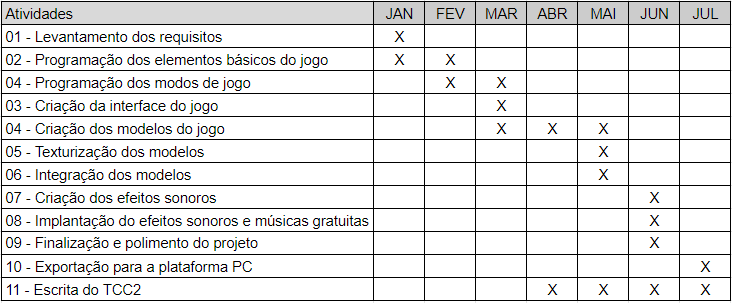
\includegraphics[scale = 0.8]{imgs/cronograma.png}%% Dimensões e localização
    
    \end{figure}

\begin{table}[]
    \centering
\begin{tabular}{|c|p{10cm}|}
  \hline
  \textbf{Atividade} & \textbf{Descrição} \\
  \hline
  01 & Levantamento dos requisitos: Será feita uma avaliação de todas as ferramentas e referências que serão utilizadas no processo de desenvolvimento. \\
  \hline
  02 & Programação dos elementos básicos do jogo: Os elementos do jogo descritos na seção \ref{subsec:coreGameplay} serão implementados. \\
  \hline
  04 & Programação dos modos de jogo: Será feita a programação específica para o funcionamento de cada modo de jogo, descrito na subseção \ref{subsec:modosDeJogo}. \\
  \hline
  03 & Criação da interface do jogo: Será implementado no motor de jogo o protótipo de interface mostrado na subseção \ref{subsec:interface}. \\
  \hline
  04 & Criação dos modelos do jogo: Os modelos 3D necessários ao jogo serão modelados. \\
  \hline
  05 & Texturização dos modelos: Os modelos 3D receberão uma textura. \\
  \hline
  06 & Integração dos modelos: Os modelos 3D serão exportados para o motor de jogos, substituindo os modelos temporários. \\
  \hline
  07 & Busca por efeitos sonoros: Será realizada a busca pelos efeitos sonoros necessários nos sites descritos na subseção \ref{subsec:audio}. \\
  \hline
  08 & Implantação dos efeitos sonoros e músicas gratuitas: As faixas de áudio serão importadas para o motor de jogos, e será feita a programação para ativação dos mesmos. \\
  \hline
  09 & Finalização e polimento do jogo: O projeto será finalizado e os detalhes finais ajustados. \\
  \hline
  10 & Exportação para as plataformas destino: O jogo será exportado para a plataforma PC \\
  %e versão para web, que será postada no site Itch.io.
  \hline
  11 & Escrita e entrega do TCC 2: Será escrito o TCC 2 abordando todas as atividades desempenhadas, para ser entregue junto ao jogo proposto. \\
  \hline
\end{tabular}
\caption{Descrição das atividades a serem desenvolvidas}
\label{tab:atividades}
\end{table}

 \section{Detalhes de implementação}\
 A escolha das ferramentas descritas na seção \ref{subsec:materiaisEMetodos} foi motivada pelo tutorial de implementação de de um jogo multiplayer 3D feito na Godot \footnote{Godot 4 - Online Multiplayer FPS From Scratch , disponível em https://www.youtube.com/watch?v=n8D3vEx7NAE}, seguido pelo autor.
 No tutorial seguido, o jogo apresenta a seguinte arquitetura,  mostrado na Figura \ref{fig:arquitetura}. Tanto os clientes quanto o servidor controlam apenas um personagem no jogo, mas têm réplicas do objeto "jogador"\space que representam todos os outros jogadores.
 Ao realizar uma ação como se movimentar, o jogo invoca a função que controla tal comportamento e aplica somente ao objeto que controla o próprio personagem. Os parâmetros que forem alterados, como por exemplo coordenadas do jogador no plano 3D, serão propagados automaticamente para os outros clientes, pelo nó de sincronização multijogador.  

 \begin{figure}[htb]
    \caption{Diagrama de arquitetura }
    \label{fig:arquitetura}%% Rótulo
    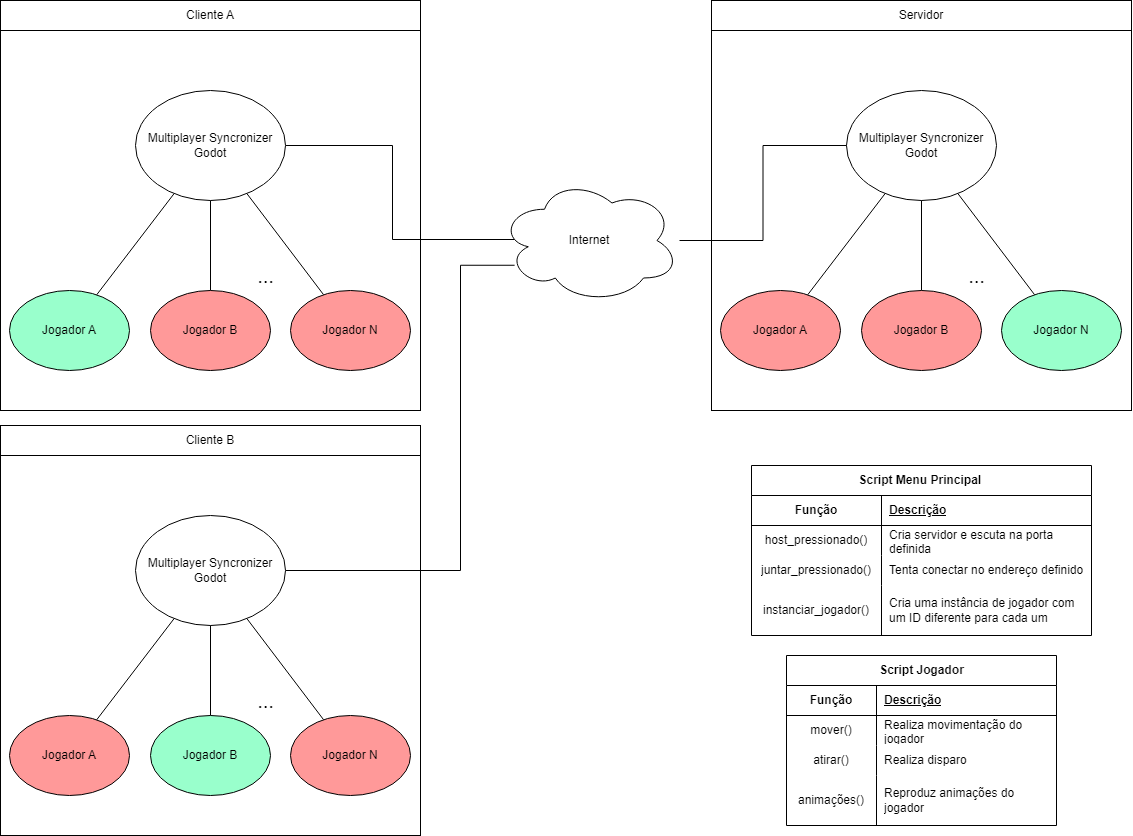
\includegraphics[scale = 0.4]{imgs/diagrama2.png}%% Dimensões e localização
    \fonte{Autoria própria}
    
    \end{figure}

O jogo será feito na arquitetura \textit{peer-to-peer}, como mostrado na Figura \ref{fig:p2p}. Será utilizado a função  de Sincronização de objetos em rede na Godot, chamada de \textit{Multiplayer Syncronizer}. Utilizando-se desse nó em conjunto com as chamadas de função RPC, podemos escrever funções que alterem o estado de um objeto, e refletir essas mudanças em todos os hosts da rede.  


% seção sobre a parte técnica
%Arquitetura do jogo (diagrama/infográfico): mais técnico, relacionando como ocorrerá o fluxo de execução do código e comunicação entre as partes (clience/servidor)
% Mencionar que fez um protótipo baseado no tutorial disponível em: ... Falar sobre esse protótipo. Colocar uma foto.
 
%%%%%%%%%%%%%%%%%%%%%%%%%%%%%%%%%%%%%%%%%%%%%%%%%%%%%%%%%%%%%%%%%%%%%%%%
% https://en.wikipedia.org/wiki/Facing_Worlds

%** INSERIR AS IMAGENS DOS PROTÓTIPO (FAZER PONTEZINHAS LIGANDO AS PEDRAS, ABRIR ESPAÇO NA TORRE POR DENTRO ( BEM GRANDE, PLAYERS SÃO PEQUENOS EM CCOMPARAÇÃO ) E UNREAL LADO A LADO.
%https://www.youtube.com/watch?v=bJxfo-nJn-o
%https://www.youtube.com/watch?v=BYbYhMNoJls&t=288s
%QD3M17 E FACING WORLDS




%
%GDD-> 
%* How does the game play ( gameplay )
%* How does the game look ( art )
%* How will the game run ( tech )
%* How will we make this game ? ( dev e business )%

%* Especificar a plataforma ( pc )
%* Descrição breve que você diria a qualquer pessoa que pergunte sobre o que é o seu jogo

%Estrutura proposta :
%*Estória :
%    * Personagem
%    * Contexto
%    * Narrativa
%*Gameyplay :
%    * Core loop gameplay
%%    * elementos e dinâmicas
 %   * Inimigos / ambiente 
%*Level Design :
%    * Progressão
%    * Objetivos
%    * Modos de jogo
%*Arte :
%    * Arte conceitual 
%    * Exemplos
%    * Áudio 
%*Outros
%    * Público alvo
%*Plano de desenvolvimento
%    * Cronograma ( falar com o professor )
%    * Ferramentas ( git, kanban...)

%--------------------- LINKS ÚTEIS ------------------
% https://mainleaf.com/pt/gdd-exemplo-e-guia-completo-para-criar-o-seu-jogo/